\documentclass[10pt]{article}
\usepackage{page_style}
\usepackage{listings}
\usepackage[export]{adjustbox}
\usepackage[bottom]{footmisc}

\lstdefinestyle{mystyle}{                   
    captionpos=b,
}
\lstset{style=mystyle}
\lstset{language=Python}


\definecolor{codegray}{gray}{0.93}
\newcommand{\code}[1]{\colorbox{codegray}{\texttt{#1}}}
% \newcommand{\code}[1]{\texttt{#1}}

% %%%%%%%%%%%%%%%%%%%%%%%%%   COMMANDS   %%%%%%%%%%%%%%%%%%%%%%%%%%%%%%%%%
\newcommand{\ts}{\textsuperscript}
\newcommand{\maxnodes}{N_{nodes-max}}
\newcommand{\dth}{D_{threshold}}


% %%%%%%%%%%%%%%%%%%%%%%%%%   HEADER   %%%%%%%%%%%%%%%%%%%%%%%%%%%%%%%%%
\title{
    \huge Project Report: Mining Data Records in Python \\ 
    \medskip
    \large Data Wrangling with Pierre Senellart \& Leonid Libkin  \\
    Master IASD - PSL University
}

\author{
    João Paulo Casagrande Bertoldo \\
    \href{mailto:joaopcbertoldo@gmail.com}{\texttt{joaopcbertoldo@gmail.com}} 
}
    
\date{April 2020}


% %%%%%%%%%%%%%%%%%%%%%%%%%   DOCUMENT   %%%%%%%%%%%%%%%%%%%%%%%%%%%%%%%%%

\begin{document}

% elements to mention
% - api 
% - extension
% - file management

% setup.py not been tested


% https://github.com/joaopcbertoldo/pymdr

% %%%%%%%%%%%%%%%%%%%%%%%%%   ABSTRACT   %%%%%%%%%%%%%%%%%%%%%%%%%%%%%%%%%
{
    \setstretch{.7} 
    \maketitle

    \begin{abstract}
    
    This project is part of the evaluation of the course \href{https://moodle.di.ens.fr/enrol/index.php?id=14}{\textit{Data Wrangling}} with Professors Pierre Senellart and Leonid Libkin as part of the \href{https://www.lamsade.dauphine.fr/wp/iasd/en/}{Master's degree IASD} at the \href{https://www.psl.eu/en}{PSL University} (session 2019/2020).
    \medskip
    
    This report presents a review on my implementation of the algorithm described by \cite{mdr} in the paper \say{Mining Data Records in Web Pages}. 

    \end{abstract}
}

\tableofcontents
\newpage

% %%%%%%%%%%%%%%%%%%%%%%%%%   BODY   %%%%%%%%%%%%%%%%%%%%%%%%%%%%%%%%%

\section{Introduction}


\section{Original Paper}

To implement this algorithm, I based myself on \cite{mdr-technical}. It was published in 2003 and, according to Semantic Scholar \citep{mdr-semantic-scholar}, this article has been cited over 400 times, of which more than 90 articles were highly influenced by it.

\subsection{Authors}

\paragraph{Bing Liu}

Liu is a Distinguished Professor of Computer Science at the University of Illinois at Chicago (UIC). He is the author of the book \emph{Web Data Mining} \citep{web-data-mining}. His main areas of interest are data mining and machine learning. He published many articles, like the one used for this project, about data mining applied to data from the web. More recently, Liu has worked and written about sentiment analysis - having published two books on the subject \citep{liu-page}.

\paragraph{Robert L. Grossman}

Robert was a professor at the university of Illinois at Chicago for over more the 20 years. Nowadays he is a professor in several departments at the University of Chicago. Grossman has received several awards and makes part of a number of advisory boards. He is, for instance, Chair of the Open Commons Consortium (OCC). Moreover, he is also an ACM Fellow since 2016 \citep{robert-page, robert-linkedin}.

\paragraph{Yanhong Zhai}

Yanhong was, by the time of the publication, a PhD student at the University of Illinois at Chicago. Since she received her PhD degree in 2006, Yanhong has been working in Microsoft. Having worked as Software Development Engineer (SDE) for more than 10 years, notably in web data mining and business inference, she is now a Principal SDE in the company \citep{yanhong-page, yanhong-linkedin}.

\subsection{Overview}

The article reports about the algorithm so called \say{Mining Data Records} (MDR). A \emph{data record} is a structured object on a page that holds information about some entity. The latter is supposedly from some database of records that is exposed via the website. For instance, a data record can be a product on a market place website like Amazon (Figure \ref{fig:pianos}).

\begin{figure}[b]
  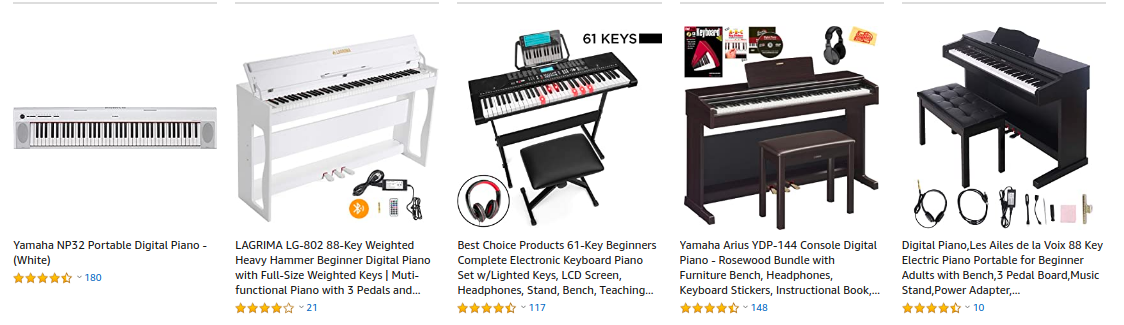
\includegraphics[width=0.9\linewidth]{fig/pianos.png}
  \caption{Sample page from \href{www.amazon.com}{www.amazon.com} with data records about pianos. Each product offered on the page is a data record - that is, an object containing an image, a title, a rating, and the number of purchases of the product.}
  \label{fig:pianos}
\end{figure}

MDR finds data records inside table tags in HTML pages without using any heuristics about the page's contents or topic. Here bellow, I briefly describe the article's contents, but the reader is encouraged to read the short \citep{mdr} or technical \citep{mdr-technical} version of the original publication for more details.


\paragraph{Rationale}

Consider an HTML document as a tree structure where tags inside another are children of the latter (see Figure \ref{fig:html-as-tree}). The core of the algorithm is based on three ideas: the notion of Generalized Node (GNode for short), Data Region (DR), and a measure of distance between GNodes. A GNode is a set of $n \in {1, ..., \maxnodes}$ HTML adjacent nodes (thus, nodes under the same parent node). A DR is a set of adjacent GNodes that are \emph{similar}. See Figure \ref{fig:gnode-and-dr} for an illustration of these two concepts.

\say{Similar}, in this context, means that the distance between each 2 directly adjacent GNodes is bellow the threshold $\dth$. The measure of distance is the Normalized Levenshtein Edit Distance \footnote{See the \cite{lev-dist-wiki} for more information.}:

\begin{equation}\label{eq:dist}
    d\left(s_{1}, s_{2}\right)=\frac{LevenshteinEditDist\left(s_{1}, s_{2}\right)}{\frac{\text {length}\left(s_{1}\right)+\text {length}\left(s_{2}\right)}{2}} \in [0, 1]
\end{equation}

The values of $\maxnodes$ and $\dth$ are parameters of the algorithm and the authors reported using, respectively, $10$ and $0.30$. Once the DRs are found in the HTML node tree, there is a last scan over them that figure out which ones are data records or not.


\begin{figure}[!b]
    \centering
    
    \begin{subfigure}[b]{.45\textwidth}
        % \centering
        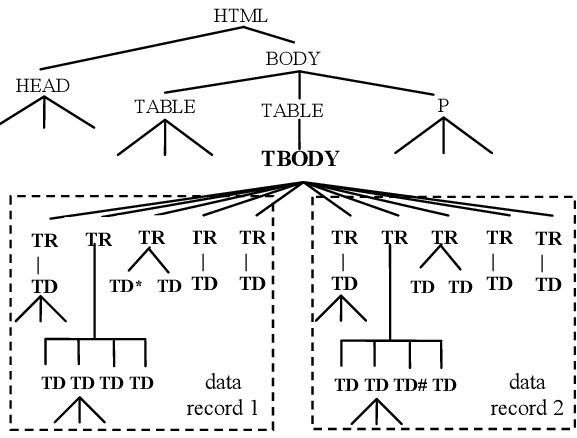
\includegraphics[width=0.95\linewidth,left]{fig/html-as-tree.png}
        \caption{HTML as a tree structure.}
        \label{fig:html-as-tree}
    \end{subfigure}
    %
    \begin{subfigure}[b]{.54\textwidth}
        
        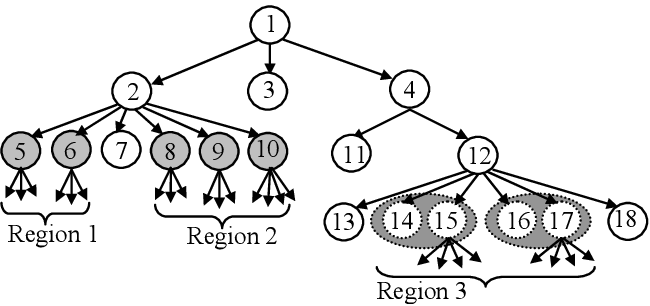
\includegraphics[width=0.95\linewidth,right]{fig/gnode-and-dr.png}
        \caption{GNode and DataRegion concepts examples.}
        \label{fig:gnode-and-dr}
    \end{subfigure}
    
    \caption{Key concepts. Source: \cite{mdr}.}
    \label{fig:html-gnode-dr}
\end{figure}


% todo: schematic here?

\paragraph{Experimental results}

The authors tested MDR on $46$ different pages, with a total of $621$ objects (data records). They reported a precision and a recall of, respectively, $100\%$ and $99.8\%$, outperforming (by far) other algorithms previously proposed by other authors. The list of websites used by them can be seen on the Table 1 in \cite{mdr}. 


\paragraph{Issues}

Unfortunately, the authors did not make available any reference implementation. They also did not make public the specific cached HTML pages that they used to test the algorithm on, or even the specific pages used (only the websites). Some of the websites mentioned in the their test set do not exist anymore (like \href{http://www.bookbuyer.com}{\textit{bookbuyer.com}} and \href{http://www.codysbooks.com}{\textit{codysbooks.com}}) or became a completely different website (such as \href{https://www.eveonline.com/}{\textit{eveonline.com}}). Moreover, they do not describe how the data was labeled or inspected, making it harder to reproduce their precision and recall metrics.



\section{Implementation}



\subsection{Overview}

The initial goal of this project was to implement an open version of the algorithm described in \cite{mdr} in Python. In addition to it, the project would include a visualization feature that would allow the user to inspect the code execution. Unfortunately, as we will see in the sections that follow, it was not possible to create a visualization. 

The first implementation of the algorithm, with the suggested parameters, did not work as the authors claim it does. For this reason, I decided to investigate the effect of some parameters and variations of the algorithm. 

In order to test my implementation, I collected HTML pages and annotated the number of data records in each of them. To facilitate the annotation task, I created a Google Chrome extension to interface with a Flask \footnote{\href{https://flask.palletsprojects.com/en/1.1.x/}{Link to Flask's official page}} web API. Next, I ran the several steps of the algorithm individually, saving intermediate results for inspection.

% todo: https://github.com/joaopcbertoldo/pymdr/tree/0.1 release 0.1 !!!!!!!!!!!!!!!!!!!!!1

% implementation + viz...
% core, utils, api
\paragraph{Code structure} The next subsections will briefly explain how the final implementation works and what are its elements (classes, functions, etc). The code referenced in the rest of this section is organized as follows\footnote{\href{https://github.com/joaopcbertoldo/pymdr}{Link to the \emph{pymdr} project's GitHub page.}}:

\begin{lstlisting}[caption=Main code structure]
# project root
/  
|--/src
|  |--/api
|  |  |-- main.py
|  |  
|  |--/extension
|  |  |-- readme.txt
|  |  |-- manifest.json
|  |   ...
|  |
|  |-- core.py
|  |-- files_management.py
|  |-- prepostprocessing.py 
|  |-- utils.py
|
|--/test 
|   ...
\end{lstlisting}



\subsection{Core}

This is where the algorithm itself and the entities (classes) that interact with it live. The code in this module is not supposed to manage any of the files, input or outputs, nor treat the way they are loaded and saved. Instead, it expects all the inputs to be in known specific formats.

The main input types are \code{HtmlElement}s (from \code{lxml.html}), the classes defined in the module (discussed next), and a few dictionary structures, which are specified with \code{typing}\footnote{\href{https://docs.python.org/3.6/library/typing.html}{Link to the typing library's page in Python 3.6}.} for documentation\footnote{\href{https://github.com/joaopcbertoldo/pymdr/blob/7ff7f7653feff23704b6b786db8499188ba378af/src/core.py\#L273}{Link to their definitions in \code{core.py} in the repository}.}.



\subsubsection{Dependencies}

\paragraph{lxml} After reading about\footnote{For instance,   \href{https://tomassetti.me/parsing-html/\#python}{this review on \emph{tomassetti.me}}.} and experimenting with a few Python libraries for HTML handling, I chose \code{lxml} for a few reasons. First, it is designed to work with the \code{ElementTree} API, making it simple to treat the HTML document as a tree structure like the original paper does. Second, it is fairly easy to parse the HTML and serialize the objects, which are the main functionalities I used. And finally, it is not full of fancy features that I did not need like other options.

\paragraph{graphviz} Since the original goal was to generate visualizations, I also reviewed several options for graph rendering and chose \code{graphviz} because it is open source and provides a fairly simple interface for the features I was looking for. In the end, it was not used in the main code, but you may find some utility functions that can be used to render a graph from an \code{HtmlElement}.

\paragraph{python-Levenshtein} One of the core tasks in the algorithm is to measure the (normalized) Levenshtein edit distance between strings - "similar" GNodes are those for which this distance is bellow a predefined threshold. I initially used the library \code{strsim}\footnote{\href{https://pypi.org/project/strsim/}{Link to \code{strsim}'s PiPy page}.}, but it started creating problems (which I could not debug) at some point. Therefore I switched to the implementation in \code{python-Levenshtein}\footnote{\href{https://pypi.org/project/python-Levenshtein/}{Link to \code{python-Levenshtein}'s PiPy page}.}.



\subsubsection{Classes} \label{txt:classes}

\paragraph{GNode}

It corresponds exactly to the concept of \emph{Generalized Node} introduced in the original paper to represent a set subsequent HTML tags in the document graph. A GNode includes all the subtrees starting at its nodes. In practice, it is referenced by the parent node's name and the 0-starting indices of the first and last nodes of the GNode.

\paragraph{DataRegion} A DataRegion is a tuple with the GNode size (i.e. the number of HTML nodes in it), the index of the first node of the first GNode, and the number of nodes covered by the GNode. This notation is not very intuitive but it is rather handy inside the algorithms that use it. For practical reasons, I also added to it the parent node's name - which is, by definition, the same as its covered GNodes' parent. 

\paragraph{DataRecord} \label{txt:class-data-record} Most of the time, DataRecords correspond exactly to one DataRegion. However, some data records might be split in more than one DataRegion, for instance when the titles of the objects are in cells of a table row and the description in the respective cells of the next row\footnote{This particular type of case is better explained in the section \say{Non-contiguous object descriptions} in \cite{mdr}}. Therefore, a DataRecord object is a list of GNodes, so both cases can be treated uniformly.

\paragraph{NodeNamer} Unfortunately, \code{lxml}'s implementation does not have a consistent \code{id()} (same for \code{\_\_hash\_\_()}). I do not know the reason, but I empirically checked that the same object might have a different result for those functions between calls (during the same run time). For this reason, it is not easy to uniquely reference any node of a generic HTML document. My solution was to add a node name as a tag attribute to the nodes themselves with a sequential value. This class serves as stateful function that is used as a shortcut to get that value from the \code{HtmlElement}s and to avoid a snippet repetition. 

\paragraph{MDR} This class is rather an utility that puts together all the pieces of the algorithm (written in functions). It makes easier to access a number of variables and mappings (the data structures described bellow) that are passed between the functions.

\paragraph{Others} During my tests, I considered using different distance thresholds for the edit distance in the different places where this notion is used (there are three of them). The class \emph{MDREditDistanceThresholds} would be used to allow this change to be made easily, but in the end it was not used. Finally, \emph{WithBasicFormat} is an utility for printing the others in a more readable way easily, in order to make it easier to debug the application.
% -- MDREditDistanceThresholds --> varying thresholds, mistake, but why it made sense
% -- WithBasicFormat --> quick comment



\subsubsection{Intermediate structures}

These two are important data structures for understanding the code because the act like mappings of information. They are used to pass sub-results between the sub algorithms.

\paragraph{DISTANCES\_DICT\_FORMAT} It keeps all the distances between pairs of GNodes, which are all computed before being used. This dictionary's keys are the node names which maps to another dictionary. This one maps the possible GNode sizes (integers from $1$ up to $\maxnodes$) to yet another dictionary. The latter maps pairs of GNodes to distances (a float between $0$ and $1$).

\paragraph{DATA\_REGION\_DICT\_FORMAT} This one maps the nodes' names the set of DataRegions found under that node.



\subsubsection{Functions} \label{txt:functions} 

The main functions correspond almost exactly to the pseudo codes described in the original paper. Their behaviors can be summarized as follows:

\begin{itemize}
    
    \item \textbf{compute\_distances}: recursively pass over all the nodes to compute the distance dictionaries;
    
    \item \textbf{\_compare\_combinations}: on a given node, effectively goes through all the possible combinations of pairs of GNodes of all sizes and computes the distances;
    
    \item \textbf{find\_data\_regions}: recursively find all the data regions under a subtree of HTML document;
    
    \item \textbf{\_identify\_data\_regions}: on a given node, find all the disconnected data regions such that each one is the largest (in terms of covered node) possible; 
    
    \item \textbf{find\_data\_records}\footnote{This algorithm is not directly given in the paper like the other, but only described in the text.}: scans all the DataRegions to extract DataRecords accordingly to two different cases: when the GNode sizes are of size 1 (with \_find\_records\_1) or larger (with \_find\_records\_n);
    
    \item \textbf{\_find\_records\_1}: creates DataRecords either from all the GNodes of the DataRegion or from its children;
    
    \item \textbf{\_find\_records\_n}: creates DataRecords directly from the GNodes covered by the DataRegion or from pieces of them to handle the case where the records are not contiguous (see the paragraph about the \nameref{txt:class-data-record} class).
    
\end{itemize}

The other functions in the module are merely auxiliary ones.



\subsubsection{Parameters}

The algorithm has three parameters that are passed to the initialization of the MDR object:

\begin{itemize}
    
    \item \textbf{minimum\_depth}: all nodes with a tree depth\footnote{\href{https://en.wikipedia.org/wiki/Tree-depth}{Link to the definition of "Tree depth" on Wikipedia}.} are not taken into consideration in the recursive calls of the functions described above. As a consequence, any direct child of these nodes can never be part of a DataRecord;
    
    \item \textbf{max\_tag\_per\_gnode} ($\maxnodes$): the largest GNode size taken into consideration;
    
    \item \textbf{edit\_distance\_threshold}: the maximum distance between two GNodes for them to be considered \emph{close} - therefore, possibly in the same DataRegion.
    
\end{itemize}



\subsection{Web API and Chrome Extension}

To make it easier to use and test \emph{pymdr}, I developed a minimalist Google Chrome extension that allows the user to call the algorithm on a (locally running) Flask API. The extension has two functionalities:  

\begin{enumerate}
    
    \item It copies and sends to the API the URL of the currently open page. Then the API executes the algorithm and returns a local file path. The file is a local copy of the HTML page with all data records painted with different colors.
    
    \item The user inputs the correct number of data records on the page and the API saves it (together with the page's URL) locally. This annotation is later used to help testing the algorithm's accuracy.
    
\end{enumerate}

The extension must be installed using Chrome's developer mode on and with a flask API running locally. To install the extension, follow the instruction on the \emph{readme} file inside the extension's folder\footnote{\href{https://github.com/joaopcbertoldo/pymdr/blob/7ff7f7653feff23704b6b786db8499188ba378af/src/extension/readme.txt\#L1}{Link to the extension's \emph{readme} file in the repository}.}. To start the API, launch the script \emph{launch-me.sh} in the root of the file\footnote{\href{https://github.com/joaopcbertoldo/pymdr/blob/7ff7f7653feff23704b6b786db8499188ba378af/launch-api.sh\#L1}{Link to the \emph{launch-me.sh} file in the repository}.}.



\subsection{Other modules} \label{txt:other-modules}

The other two modules are rather for support tasks like managing files and pre-treating the HTML files. They are mostly used in the API and in the script used to process all the pages (more details in the next sections). 

\paragraph{Files management} 

This module gathers utilities to write/read from files and get the their paths easily. The organization of the files mostly depends on the class \code{PageMeta}, which is used to access metadata from an annotated page. All the files are referenced by a (shortened) hash of the URL of the raw HTML page where they come from. They are all located in a directory \emph{outputs} in the root of the project by default. This directory's location can be changed in the file \emph{config.yml} in the root of the project.

\paragraph{(Pre \& Post)-Processing}

The functions in this module are basically wrappers around each sub-algorithm that compose MDR (explained in the Section \nameref{txt:functions}). They save intermediate results in files, load them from previous steps, and sure that the files already processed are skipped. This is useful to execute the test script used to investigate the factors that influence the algorithm so that the executions are consistent between calls.



\subsection{Unit tests}

The directory \emph{test} (see has the same structure than \emph{src} and the respective files contain unit tests for those in \emph{src}. They use Python's builtin package \code{unittest}. For maintenance purposes, I did not create unit tests for everything, but only for the most important parts of the algorithm. They were indeed very useful during my iterations of the code making sure to keep the code correct. 

These tests have rather simple input/output test. So, it might be a useful entry point to understand what each function is supposed to do and the data formats. 



\section{Experiments}

From the very beginning, I realized it would be painful to test and inspect the results by managing the inputs and outputs of the core module manually. For this reason, I wrote the first version of the extension and the API only for caching the HTML pages, executing MDR, and returning another file with colored HTML tags to identify the data records.

\paragraph{(Very) Slow first results} 

My very first tests showed that my code was extremely slow. Although I did not record execution times, the typical execution was at the tens of seconds or even minutes. This is way above the author's claims of sub-second execution times. Because of the slow execution times, I decided to start collecting pages and caching them for later execution. 

After re-reading the technical paper carefully, I realized that the algorithm is only supposed to consider table-related tags (table, tr, th, td, ...). In addition to that, the results did not seem correct at all. The algorithm was not capable of identifying any data record. This made sense because the algorithm was simply not intended to work with all the tags. 

To address this matter, I created a simple filter to ignore all other tags. It vastly accelerated the execution to a few seconds in the worst case. However, many of pages did not have any data record at all. After manually inspecting a few examples, I realized that many of the pages simply did not use table tags, but lists (ol and ul) for organizing the data records. 

My hypothesis is that web pages, today, use table tags way less often today. According to \cite{tables-basics}: \say{...a lot of people used to use HTML tables to lay out web pages...}. This essentially affects the algorithm's assumptions because it is specifically made to work well with these tags. Therefore, I decided to make sure it was not a matter of bad parameters. So I tested the algorithm with different threshold values, since this is the most important parameter, in addition to a few variations. 



\subsection{Analyzed factors}

The following paragraphs explain the different variations of the algorithm that I tested.

% - table elements only --> cutting off for performance in computing distances
% - table elements only --> too little results
% -- manual check that there are not many tables
% -- later confirmed in the results viz

\paragraph{Threshold}

The original recommended value was of $0.30$, so it makes sense to keep the threshold range \emph{around} $0.30$. Also, as I informally observed, the slowest part of the algorithm (by far) is the distance computation (see \nameref{txt:functions}). This part of the algorithm is independent of the threshold choice, which means that having a large value set for this parameter should not slow down the tests execution so much. So I tested with all the values in ${0.05, 0.06, ..., 0.49, 0.50}$.

\paragraph{HTML Lists} 

MDR was designed to work well on pages that use table tags, so taking all the HTML tags into consideration did not make any sense. On the other hand, taking the authors' same assumption and only taking into consideration the table tags seemed too restrictive. Thus, I decided to consider both a version only with tables and another with lists additionally. This behavior can be controlled by changing the function \code{should\_process\_node} in \emph{core.py}.

\paragraph{Edit distance distortion}

While reviewing and cleaning my code, I realized that I could have introduced an issue to the algorithm by distorting the edit distances. This happened due to the naming solution (see the class NodeNamer in the section \nameref{txt:classes}) I used to reference the nodes. Since it adds a new attribute to the tags. While serializing subtrees this attribute ends up being part of the string. This affects the distance measure especially for nodes with little content because the sizes of the attribute's key and value make the distances decrease artificially. 

For this reason, I made a hot fix that cleans all the attributes from the subtrees before measuring the distances. The parameter used to control this behavior is the constant \code{STR\_DIST\_USE\_NODE\_NAME\_CLEANUP} in \emph{core.py}.

Therefore, there are 4 tests: $\{\text{with lists}, \text{without lists}\} X \{\text{with correction}, \text{without correction}\}$ (where \say{correction} refers to the distance distortion fix). For each of those, I tested all the threshold values, looked up for the best values, and inspected some \emph{promising} results manually in detail.



\subsection{Procedure}

\paragraph{Test pages}

% - cached pages not available --> certainly aged up
% - pages that do not exist anymore --> had to verify myself
% - did not give exact urls --> i picked some random ones

First, I collected sample pages from the same websites mentioned in \cite{mdr}\footnotemark. Several of them did not exist or completely changed of domain/content. In total, I collected $94$ pages, of which $86$ were processed - the others went through some problem in the process and then were ignored. I collected these pages using the Chrome extension and annotating the ground truth number of data records on the page. The pages' URLs and their annotations can be seen in the file \emph{outputs/pages-meta.yml}.

\footnotetext{I looked for the original cached pages used by the authors and even tried to get in touch with them to find them. Unfortunately I could not find them out. I also tried to look up for the pages used in the two main references of the paper (OMNI and IEPAD), but they are also not available.}

\paragraph{Script}

I used the script in \path{dev/training/preprocess_all.py} to go through all the thresholds, all the pages, step by step. To control the other parameters, one should directly change the code in \path{core.py}. It is possible to choose, directly in the script, which steps should be executed to avoid useless executions when running it multiple times.

\paragraph{Outputs}

The results and intermediate files generated by the script are organized in the folder \path{outputs} under the root of the project. This is due to the \path{file_management.py} module and can be changed via the file \path{config.yml} in the root of the project (see the section \nameref{txt:other-modules} for more information). The folder contains the following sub directories: 

\begin{itemize}

    \item \path{raw\_htmls}: contains the cached HTML pages without any modification;
        
    \item \path{preprocessed\_htmls}: contains HTML files after two phases of preprocessin: (1) without comments, script, and style tags; (2) with the node names added to all the tags (see \code{NodeNamer} in \nameref{txt:classes}).
        
    \item \path{intermediate\_results}: 
        
    \item \path{results}: 
    
\end{itemize}



\subsection{Results}

\paragraph{Evaluation}

% - no precise description of tagging/labelling --> how to measure precision/recall? --> simplified way of counting to investigate --> coloring the background for visual inspection

\paragraph{Reproduction}

% nb with comments
% evaluating_stuff-with-list-with-cleanup.ipynb


% would have chosen another framework if I knew the id issue...


% %%%%%%%%%%%%%%%%%%%%%%%%%   REFS   %%%%%%%%%%%%%%%%%%%%%%%%%%%%%%%%%
\newpage
\bibliography{refs} 


\end{document}